\documentclass[12pt]{article}
\usepackage[a4,margin=0.5in]{geometry}
\usepackage{xcolor}
\usepackage{graphicx} % Required for inserting images
\usepackage{tabularx}

%\title{bubble Dynamics}
%\author{B.H.T Goh}
%\date{\today}

\begin{document}
%\maketitle
\begin{center}
\color{violet}

   \Large{\textbf{ME5470 : Introduction to Parallel Scientific Computing}}\\
   \Large{\textbf{Assignment-01}}\\
   \color{red}
   \vspace{5pt}
   \Large{\textbf{Yashwant Singh}}\\
   \Large{\textbf{(ME22RESCH11009)}}
    
   %\section{Introduction}
\end{center}
\hrule
\vspace{15pt}
\par Q1(a).

\begin{table}[h]
  \centering
  \caption{File size of ASCII and Binary in MB}
  \vspace{10pt}
  \begin{tabular}{|m{2cm}|m{3.6cm}|m{3.7cm}|}
      \hline
     Matrix size & ASCII file size (MB) & Binary file size (MB) \\
      \hline
      4000 & 319.956203 & 122.070312 \\
      \hline
  \end{tabular}
  \label{tab:collapse_behavior11}
\end{table}

Q1(b).

\begin{table}[h]
  \centering
  \caption{File size of ASCII and Binary in MB}
  \vspace{10pt}
  \begin{tabular}{|m{2cm}|m{2cm}|m{2cm}|m{2cm}|m{2.8cm}|m{2.8cm}|}
      \hline
     Matrix size & Memory size (MB) & ASCII file size (MB) & Binary file size (MB) & ASCII/Memory & Binary/Memory\\
      \hline
      1 & 8E-06 & 1.8E-05 & 8E-06 & 2.375 & 1 \\
      \hline
      5 & 0.000191 & 0.000434 & 0.000191 & 2.275 & 1 \\
      \hline
      25 & 0.004768 & 0.011296 & 0.004768 & 2.369 & 1 \\
      \hline
      125 & 0.119209 & 0.293274 & 0.119209 & 2.46016 & 1 \\
      \hline
      625 & 2.980232 & 7.475991 & 2.980232 & 2.508526 & 1 \\
      \hline
      3125 & 74.505806 & 195.098538 & 74.505806 & 2.618568 & 1 \\
      \hline
      4000 & 122.070312 & 319.956203 & 122.070312 & 2.621081 & 1 \\
      \hline
  \end{tabular}
  \label{tab:collapse_behavior11}
\end{table}

\begin{figure}[h]
    \centering
    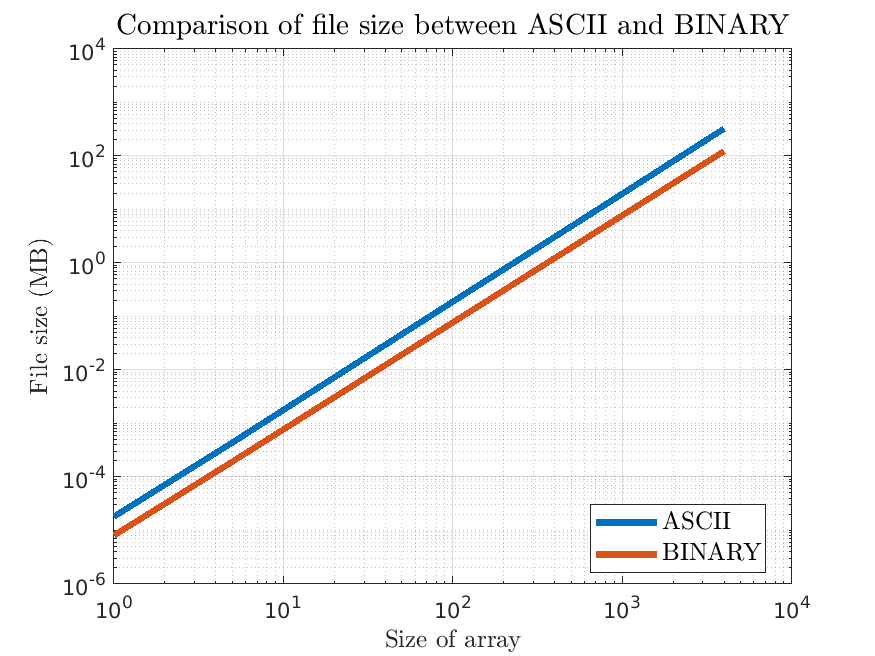
\includegraphics[scale=0.8]{Comparison_of_file_size_between_ASCII_and_BINARY.png}
    \caption{File size comparison between ASCII and Binary}
    \label{fig:enter-label}
\end{figure}



\end{document}
